\section{Methods}

%\subsection{TGS Methods}
% Include specific details about TGS methods here.

\subsection{Elastodynamic Methods}
Following the approach by Du (2017), materials are modelled as anisotropic unbounded media through which elastic waves propagate according to the elastodynamic wave equation:

\begin{equation}
    C_{ijkl} \frac{\partial U_l(\vec{r},t)}{\partial x_j\partial x_k}= \rho(\vec{r},t)\frac{\partial^2 U_l(\vec{r},t)}{\partial t^2}
    \label{eqn:ewe}
\end{equation}

where $C_{ijkl}$ are fourth-order stiffness tensor entries that are permutatively indexed by $i,j,k,l=1,2,3$, $\rho$ is density, and $U$ is the wave function.

The elastic tensor is calculated using a variable cell relaxation algorithm that consists of a loop over iterative SCF calculations while adjusting atomic positions and lattice constants. Elasticity theory relates the strain applied to the unit cell to the resulting calculated stress as an inverse problem, which could be solved using a non-linear solver with prior data as an initial guess vector. Deterministic thermoelastic relationships are also used to calculate elastic tensors from changes in total energy and volume using \textit{ab initio} stress calculations. Both methods are used in a self-consistent fashion to converge to a solution that solves the elasticity inverse problem, $\underline{C}\vec{\epsilon} = \vec{\sigma}$, as follows: \cite{timoshenko1951theory, mit1620}



\begin{equation} \label{eqn:stiffness-full-notation}
\begin{bmatrix}
C_{1111} & C_{1122} & C_{1133} & C_{1123} & C_{1113} & C_{1112} \\
 & C_{2222} & C_{2233} & C_{2223} & C_{2213} & C_{2212} \\
 &  & C_{3333} & C_{3323} & C_{3313} & C_{3312} \\
 &  &  & C_{2323} & C_{2313} & C_{2312} \\
 & symm &  &  & C_{1313} & C_{1312} \\
 &  &  &  &  & C_{1212} 
\end{bmatrix} \begin{bmatrix}
\epsilon_{11} \\
\epsilon_{22} \\
\epsilon_{33} \\
2\epsilon_{23} \\
2\epsilon_{13} \\
2\epsilon_{12} 
\end{bmatrix}  =  \begin{bmatrix}
\sigma_{11} \\
\sigma_{22} \\
\sigma_{33} \\
\sigma_{23} \\
\sigma_{13} \\
\sigma_{12} 
\end{bmatrix}  
\end{equation} 
or in Voigt notation:
\begin{equation} \label{eqn:stiffness-voigt-notation}
 \begin{bmatrix}
C_{11} & C_{12} & C_{13} & C_{14} & C_{15} & C_{16} \\
 & C_{22} & C_{23} & C_{24} & C_{25} & C_{26} \\
 &  & C_{33} & C_{34} & C_{35} & C_{36} \\
 &  &  & C_{44} & C_{45} & C_{46} \\
 & symm &  &  & C_{55} & C_{56} \\
 &  &  &  &  & C_{66} 
\end{bmatrix}  \begin{bmatrix}
\epsilon_{1} \\
\epsilon_{2} \\
\epsilon_{3} \\
\epsilon_{4} \\
\epsilon_{5} \\
\epsilon_{6} 
\end{bmatrix}  =  \begin{bmatrix}
\sigma_{1} \\
\sigma_{2} \\
\sigma_{3} \\
\sigma_{4} \\
\sigma_{5} \\
\sigma_{6} 
\end{bmatrix}  
\end{equation}

\begin{figure}[h!]
    \centering
    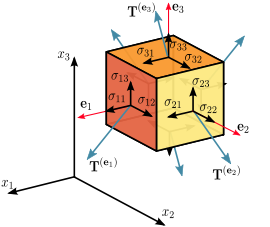
\includegraphics[width=0.6\textwidth]{Parts/Figures/Cij.png}
    \caption{Stress tensor visualization. (Source: S.A.F. Al Dajani. S.M. Thesis.)}
    \label{fig:seis-refl-tech}
\end{figure}

\subsection{DFT Methods}
Material properties are calculated from a self-consistent, non-linear field calculation, (Fig. \ref{fig:scf-loop}) which is a variational method that optimizes over charge density that adjusts atomic positions until a threshold in energy minimization is achieved in a simplified ion-core model of atoms and electrons in a given material to solve the many-body wave equation. \cite{Schwingenschloegl2004} Electron dispersion is calculated using a non-consistent field calculation to interpolate the energy calculations in momentum space. The phonon dispersion is calculated from the dynamical matrix obtained from \textit{ab initio} calculations. \cite{hung2022quantum, giustino2014materials}

Self-consistent, non-linear field calculation algorithms calculate external potentials with a Poisson equation solver, (Fig. \ref{fig:scf-loop}) which depends on simulation geometry, atomic positions of ions, pseudopotentials used for the atoms involved, and other inputs. This external potential [REF] is then used as a guess for the electron density with a Schr\"{o}dinger equation solver, [REF] which is then used as inputs to a self-consistent field loop that calculates the charge density iteratively to minimize the total energy. The accuracy of this algorithm depends on the cut-off applied to the energy minimization, the charge density, the size of the momentum grid, and other convergence thresholds on the outputs. \cite{hung2022quantum, Schwingenschloegl2004, giustino2014materials}

In order to model the BCC Fe--Cr $\delta$--ferrite solid solution, the sequential quasirandom structure (SQS) methodology was employed \cite{VandeWalleLiu2013}. 
The \texttt{mcsqs} software package within the Alloy Theoretic Automated Toolkit (ATAT) was used in order to generate SQS supercells.
The Vienna \textit{ab initio} Simulation Package (VASP) was used to perform the density functional theory (DFT) total energy calculations, which were used to derive the elastic properties as well as the enthalpy of mixing. 
Spin--polarized DFT calculations were performed on 40--atom SQS supercells employing $\Gamma$--point sampling of reciprocal space along with a 500 eV planewave cutoff energy. 
The Projector--Augmented Wave (PAW) method was employed for the ionic pseudopotential, and the Perdew--Burke--Ernzenhoffer parameterization of the Generalized Gradient Approximation (GGA) of the exchange--correlation functional. 

\subsection{Analysis of DFT Results}
With the elastic tensor obtained from quantum mechanical calculations, elastic moduli could be calculated. The significance of elastic moduli in characterizing material behavior is highlighted, and the elastic constants of iron-chrome with increasing chromium content are reported using density functional theory. By considering embrittlement criteria, the propensity of materials to undergo embrittlement could be evaluated to assess their mechanical stability.

\begin{eqnarray}
    C' = \frac{C_{11}-C{12}}{2} \\
    B = \frac{C_{11} + 2C+{12}}{3} \\
    \Rightarrow C_{11}= \frac{3B+4C'}{3} \\
    \Rightarrow C_{12} = C_{11} - 2 C' \\ \\
    G_V = \frac{C_{11}-C_{12} + 3C_{44}}{5} \\
    G_R = \frac{5(C_{11}-C_{12})C_{44}}{4C_{44}+3(C_{11}-C_{12})} \\ \\
    G = \frac{G_V + G_R}{2} \\
    E = \frac{9BG}{3B+G} \\
    \nu = \frac{3B-E}{6B}
\end{eqnarray}

Thermal properties are described by the Debye model and a lower limit for the thermal conductivity was derived at high temperatures, such that: \cite{clarke2003materialsselection,clarke2003materialsdesign}

\begin{eqnarray}
    \kappa &=& \frac{1}{3} C_v v_m \Lambda \\ \label{eqn:kappa-debye}
    \kappa_{min} \rightarrow k_B v_m \Lambda \rightarrow k_B v_m \Lambda_{min} &=& A k_B (\frac{N_A m}{M})^{\frac{2}{3}} \rho^{\frac{1}{6}} E^{\frac{1}{2}} \label{eqn:kappa-min-debye} \\
    \Theta_D &=& \frac{2\hbar v_m}{a_0 k_B} \rightarrow B \frac{\hbar}{k_B} (\frac{N_A m}{M})^{\frac{1}{3}} \frac{E^{\frac{1}{2}} }{\rho^{\frac{1}{6}}} \label{eqn:debye-temp-debye}
\end{eqnarray}
where $\kappa$ is thermal conductivity, $\theta_D$ is the Debye temperature, $C_V$ is the heat capacity at constant volume, $v_m$ is the average acoustic velocity, $\Lambda$ is the phonon mean free path, $m$ is the number of atoms, $M$ is the mass, $\rho$ is the density, $E$ is the elastic Young's modulus, and $A, B$ are correlation constants approximated from the relationship between the mean acoustic velocity and ratio of $\sqrt{\frac{E}{\rho}}$, which is valid for a wide range of Poisson ratios without loss of accuracy. The value for $A$ used for these constants are taken as $0.87 \pm 0.02$. Other studies calculate thermal conductivity using the Einstein model, which enables calculating thermal properties as a function of temperature, such that: $\kappa_{min} (T) = (\frac{\pi}{6})^{\frac{1}{3}} k_B n^{\frac{2}{3}} \sum\limits_{i} v_i (\frac{T}{\Theta_i})^2 \int\limits_{0}^{\frac{\Theta_i}{T}} dx \frac{x^3 e^x}{(e^x -1)^2}$ where $\Theta_i = v_i (\frac{\hbar}{k_B} (6\pi^2n)^{\frac{1}{3}} $. \cite{cahill1992lower}

% Include your equations for Rayleigh wave and acoustic wave frequencies here

%\subsection{Embrittlement Prediction}
% Placeholder for embrittlement prediction methods.

%\subsection{Stiffening Prediction}
% Placeholder for stiffening prediction methods.

%\subsection{Inferring Plasticity from Elasticity with Melting Point}
% Placeholder for methods to infer plasticity from elasticity.

%\subsection{Probability Distribution Methods}
% Placeholder for probability distribution methods.

% Uncomment and modify the following section if necessary
% \subsection{Additional Computational Methods}
% Spin polarized first--principles density functional theory (DFT) calculations were conducted using the Vienna \emph{Ab initio} Simulation Package (VASP). 
